\section{엔진 런타임 검증 및 실증 결과}\label{sec:eval}
본 절은 게임 엔진 보장에 초점을 맞춘 비혼합 2계층 평가를 제시한다: (i)~유한 권한 그래프·헤드리스 Godot~4.7.1 장기 실행·Datalog 스케일링을 다루는 0-LLM 결정론적 검증과, (ii)~직접 HTTPS Anthropic Claude~5.5 API 인증 스위트(\textbf{P15}--\textbf{P17}: Haiku·Sonnet·Opus~5.5 총 2.25M 토큰, deprecated \texttt{temperature} 생략 및 \texttt{output\_config.json\_schema} 적용) 및 3모델군 CLI(\textbf{P11}--\textbf{P14}, 실패 전량 보존)이다. 미실행 코호트(0/180 \texttt{20261103}, 인간 플레이테스트 \texttt{TR01--TR06} $N{=}0$)는 엄격히 분리한다.

\subsection{헤드리스 엔진 장기 실행, 권한 경계 및 Datalog 스케일링}\label{sec:tog-det}
신경망 정책 연결 전 버전 관리 엔진 브리지(\texttt{sealed\_\allowbreak lighthouse\_\allowbreak machine.gd} 및 최대 8방·3역할 5월드)를 검증하였다. 1,664건 유한 그래프 감사에서 의미 게이트는 \textbf{0/416} 위험 커밋·0/156 오거부·128/260건 $\rho$ 수리(목표 252/416 대 124/416)를 기록했고, \textbf{A1}(위험 0/1,408, 충돌 가드 128/128)·\textbf{A2}($N{=}2000$ p95 $\le$0.0751\,ms)·\textbf{A3}(4,656/4,656 결함 탐지)·헤드리스 Godot~4.7.1 장기 실행 \textbf{A4}(거부 코드 9/9·상태 격리 11/11·200에피소드 1,600/1,600틱 일관성·\texttt{step\_commit} p95 \textbf{0.708\,ms} [60\,Hz 16.6\,ms 예산 내]·정적 변화 $-268$\,B·누출 0; 그림~\ref{fig:engine-cutscenes})을 확인하였다. 480건 절차적 Datalog(\textbf{P9}, 표~\ref{tab:tog-datalog})에서 \texttt{nesy\_game.multihop}만 $\le$7.12\,$\mu$s로 100.0\% 일치하였다($Q{=}1100.19$).

\begin{figure*}[!tbp]
\centering
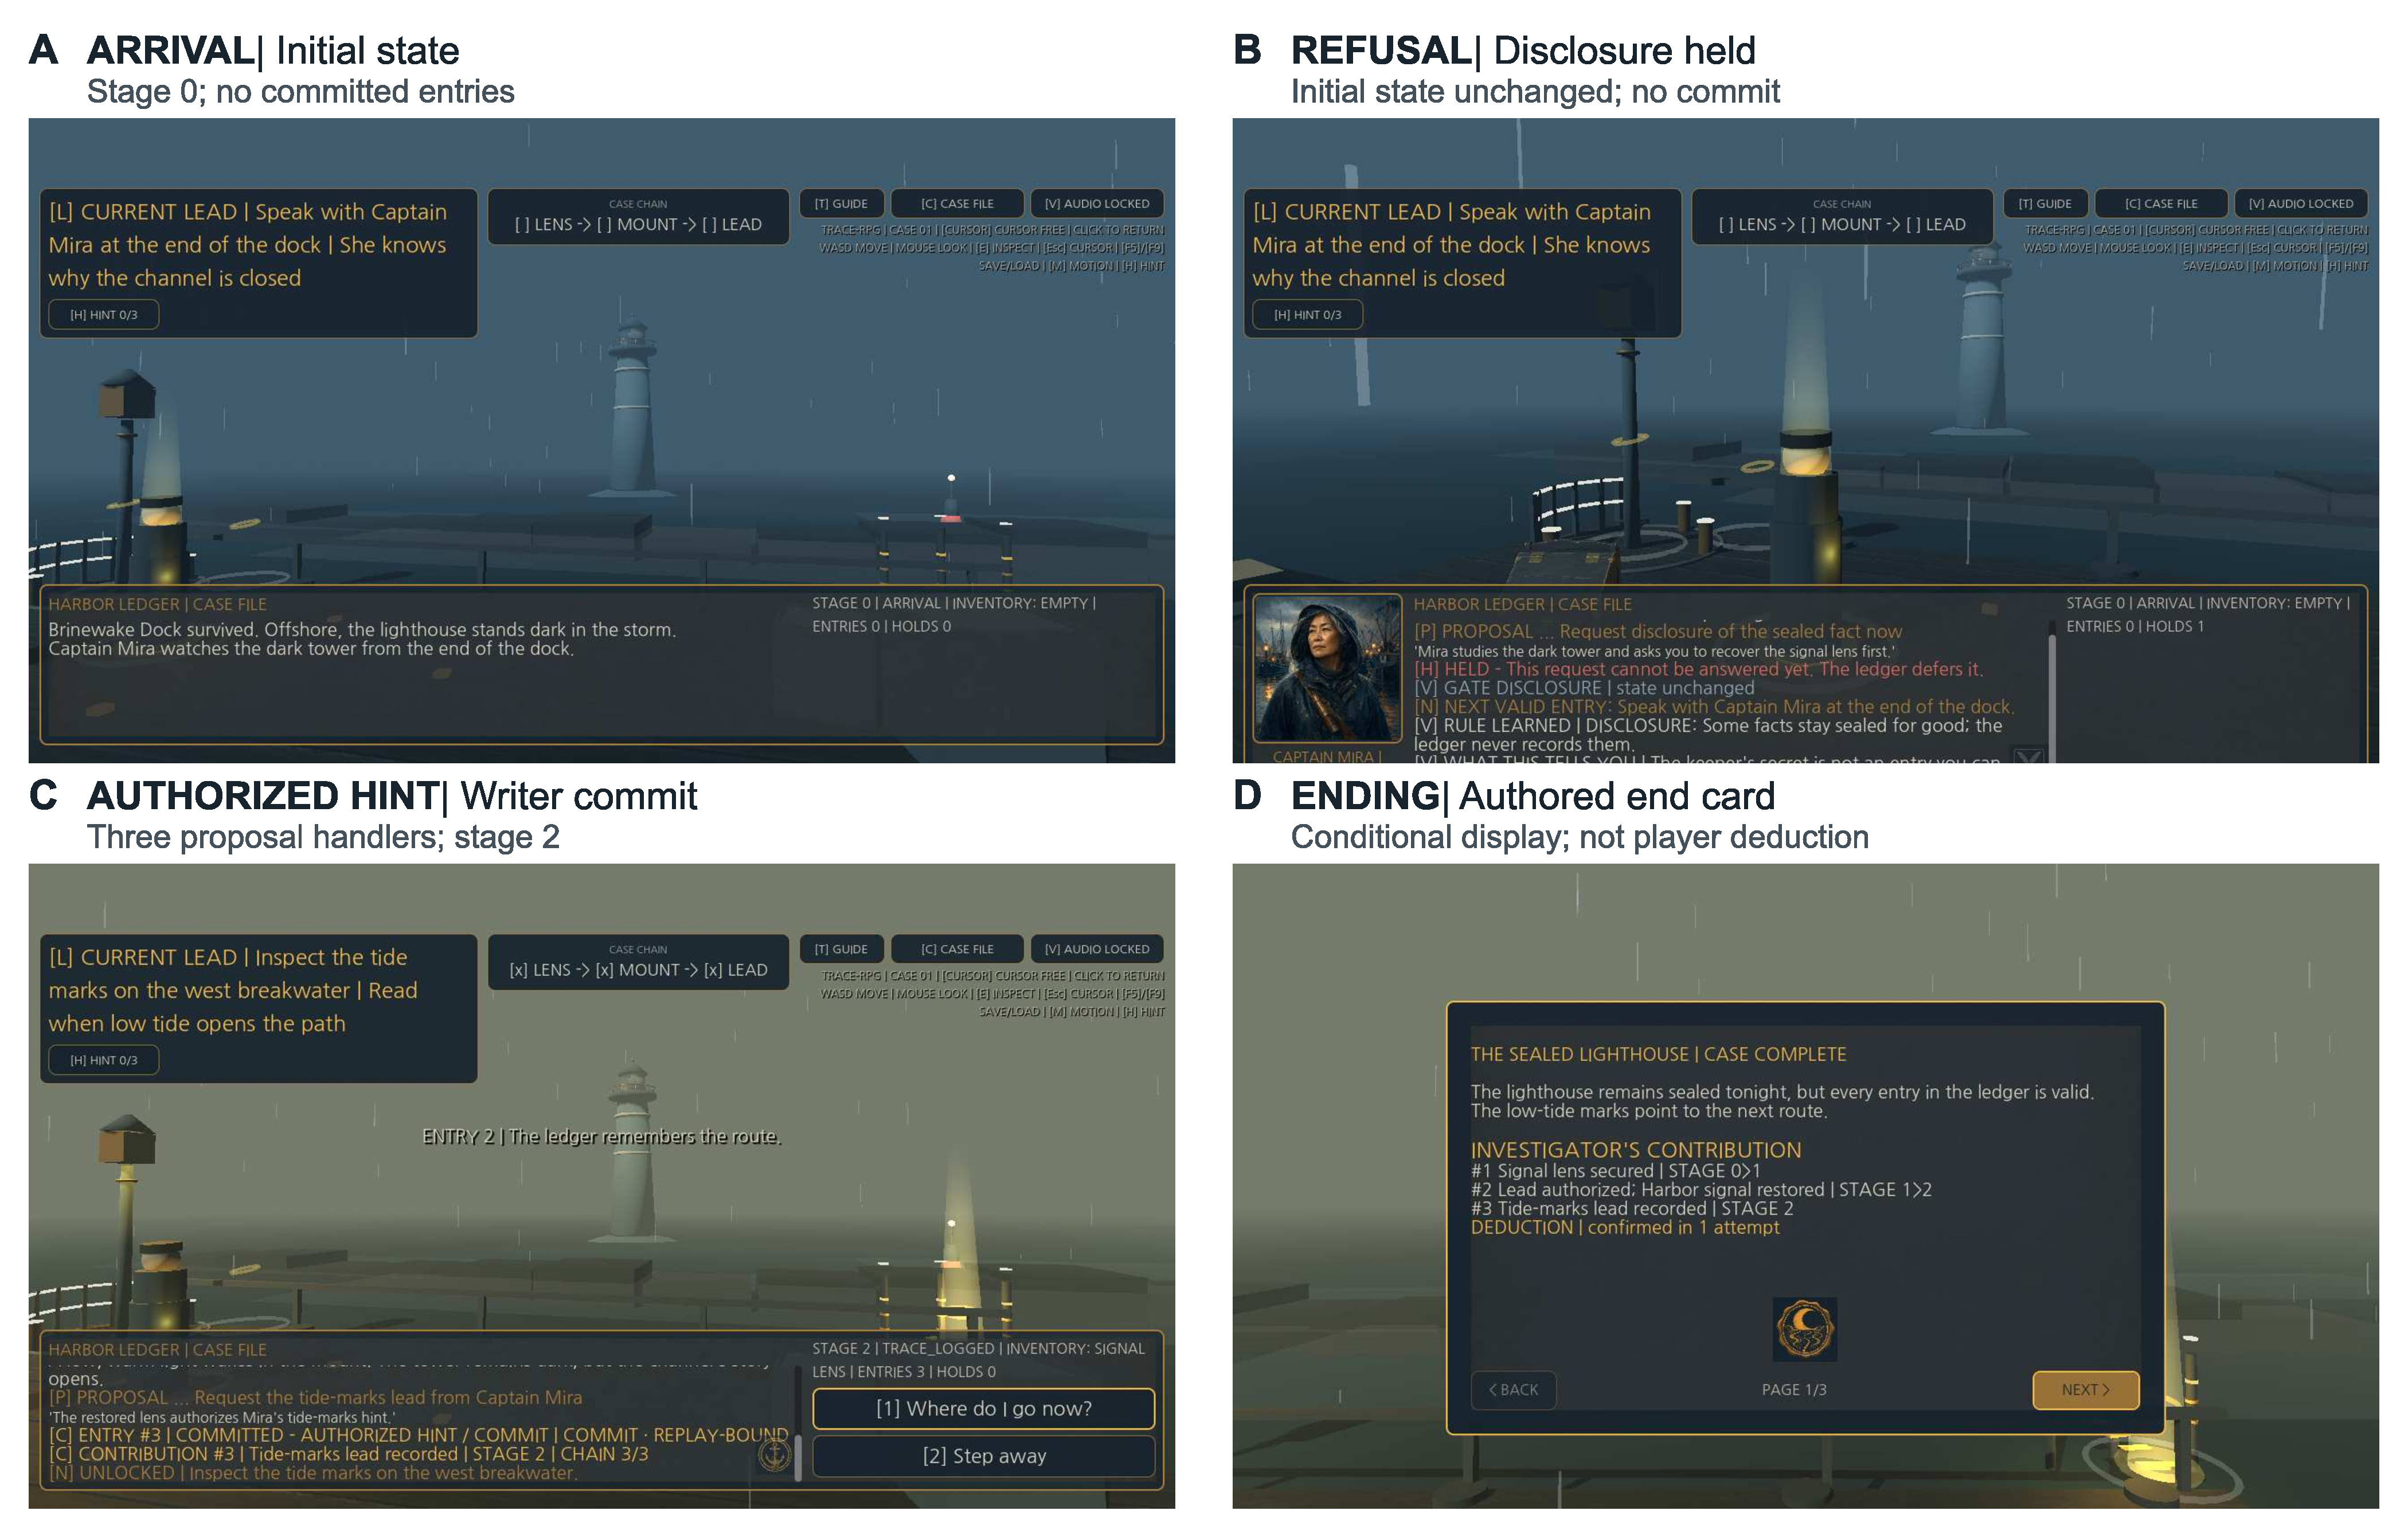
\includegraphics[width=0.90\textwidth]{../../figures/fig_engine_cutscenes.pdf}
\caption{네이티브 Godot~4.7.1 엔진 상태 머신 캡처: (A)~초기 도착, (B)~정본 상태 불변 비밀 공개 거부, (C)~2단계 인가 힌트, (D)~조건부 종료 카드.}
\Description{네이티브 Godot 4.7.1 4분할 스크린샷: 초기 도착, 비밀 공개 거부, 2단계 힌트, 조건부 종료 화면.}
\label{fig:engine-cutscenes}
\end{figure*}

\begin{table}[!tbp]
\caption{엔진 게이트 지연 및 다중 홉 오라클 스케일링 (\textbf{P9}: 480건, 0-LLM)}
\label{tab:tog-datalog}
\centering
\scriptsize
\setlength{\tabcolsep}{3pt}
\begin{tabularx}{\columnwidth}{@{}lcccc@{}}
\toprule
\textbf{검증기 구성} & \textbf{정확도 (480)} & \textbf{누출} & \textbf{중앙값 ($\mu$s)} & \textbf{p95 ($\mu$s)} \\
\midrule
\texttt{schema\_only} / \texttt{affordance} & 16.67\% (80) & 400 & --- & --- \\
\texttt{flat\_1hop\_gate} & 46.67\% (224) & 256 & 0.87--1.57 & 1.37--2.18 \\
\texttt{bounded\_2hop\_gate} & 60.00\% (288) & 192 & 1.88--2.58 & 2.66--3.91 \\
\texttt{nesy\_game.multihop} & \textbf{100.0\% (480)} & \textbf{0} & \textbf{6.46--7.12} & 9.83--11.42 \\
\bottomrule
\end{tabularx}
\end{table}

\subsection{라이브 Godot~4.7.1 폐루프 엔진 리플레이 (\textbf{P16B} 및 \textbf{P13})}\label{sec:tog-godot}
표~\ref{tab:tog-godot}는 인증 API(\textbf{P16B}: Haiku·Sonnet·Opus~5.5 21에피소드, 169,071토큰) 및 3모델군 CLI(\textbf{P13}: 42에피소드)의 Godot~4.7.1(\texttt{4.7.1.\allowbreak stable.\allowbreak official.\allowbreak a13da4feb}) 종단간 실행을 정리한다. 전량 \textbf{21/21} API 및 \textbf{42/42} CLI 에피소드가 0-LLM 헤드리스 Godot 재실행을 100\% 통과하며 위험 커밋·비밀 유출이 \textbf{0/63}이었다. 실제 제품 \texttt{SealedLighthouseMachine}에서도 API \textbf{6/6 (100\%)} 전량이 \texttt{EXACT\_\allowbreak TERMINAL\_\allowbreak HASH}(\texttt{4b231017...})에 도달했다(Godot 251.64--1009.78\,ms 대 API 9.1--40.9\,s).

\begin{table}[!tbp]
\caption{헤드리스 Godot~4.7.1 폐루프 리플레이 및 지연 분해 (\textbf{P16B} 21 API + \textbf{P13} 42 CLI)}
\label{tab:tog-godot}
\centering
\scriptsize
\setlength{\tabcolsep}{2.2pt}
\begin{tabularx}{\columnwidth}{@{}>{\raggedright\arraybackslash}X*{5}{c}@{}}
\toprule
\textbf{Godot 트랙 / 모델 계층} & \textbf{목표} & \textbf{리플레이} & \textbf{누출} & \textbf{GD (ms)} & \textbf{API (s)} \\
\midrule
\textbf{P16B} 5월드 Haiku~5.5 & 5/5 & 5/5 & \textbf{0/5} & 757--1010 & 10.6--20.9 \\
\textbf{P16B} 5월드 Sonnet~5.5 & 4/5 & 5/5 & \textbf{0/5} & 252--1005 & 14.5--36.0 \\
\textbf{P16B} 5월드 Opus~5.5 & 4/5 & 5/5 & \textbf{0/5} & 253--1009 & 16.2--40.9 \\
\textbf{P16B} 제품 \texttt{SealedLighthouse} (6) & \textbf{6/6} (해시) & 6/6 & \textbf{0/6} & 751--779 & 9.1--16.5 \\
\textbf{P13} 3모델군 5월드 (30) & 23/30 & 30/30 & \textbf{0/30} & --- & CLI \\
\textbf{P13} 3모델군 제품 \texttt{Sealed} (12) & 9/12 (해시) & 12/12 & \textbf{0/12} & --- & CLI \\
\bottomrule
\end{tabularx}
\end{table}

\subsection{폐루프 다중 에이전트 실딩, 요인 절단 및 우회 검증 (\textbf{P15}, \textbf{P16A}, \textbf{P12}, \textbf{P17})}
\textbf{P15}(Haiku·Sonnet·Opus~5.5$\times$5월드$\times$7암 105에피소드, 1,048,803토큰, \textbf{105/105} 리플레이; 표~\ref{tab:kbs-mas})에서 Safe-RL 프록시~\cite{alshiekh2018shield}(목표 0/15, 위험 16/61)와 NeMo 프록시~\cite{rebedea2023nemo}(1/15, 15/61)는 다중 홉 누출을 놓쳤고, 평면 1홉도 3/15에피소드 4/66턴(\texttt{ivory-citadel-v1} 1에피소드 2턴, \texttt{glass-foundry-v1} 2에피소드 2턴)을 누출했다. 반면 \texttt{nesy\_game.multihop} 전 암은 \textbf{15/15 (100\%)} 무누출·\textbf{0} 위험을 유지했고, \texttt{rho\_k2}에서는 거부 18건 전부가 정리~2 상태 의존 거부여서 $\rho_{\mathrm{repairs}}{=}0$으로 무세탁을 실증했으며(14/15 대 13/15는 독립 1턴 표본 변동), 하이브리드 $\rho{+}\text{LLM}_{K=1}$은 20회 안전 재선정으로 \textbf{15/15 (100\%)} 목표를 달성했다($Q_{\mathrm{goal}}{=}68.71$). \textbf{P16A}(60에피소드, 673,869토큰)에서는 정책·단계 결함에 대해 $\rho$가 \textbf{22건 라이브 수리}(Haiku 18, Sonnet 4)를 실행해 30/30 무누출·11/30 목표를 달성했고(대조 \texttt{general\_rule} 22/30·9위험), \textbf{P12} 27결함 $(a,E)$ 수리도 $\rho_{K=2}$ \textbf{27/27}(0토큰) 대 LLM 26/27(530k--542k토큰, $p{=}1.0$)이었다. 통합 540회 한·영 우회(\textbf{P17}: $\kappa{=}0.8813$, 0\% FRR, 19--29/36 명시 토큰 누락으로 Stage-1+Stage-2 상보성 입증; \textbf{P14} $\kappa{=}0.9367$)와 \texttt{DATASHEET\_v5.md}~\cite{gebru2021datasheets}·Croissant~1.0 v5~\cite{akhtar2024croissant}로 아티팩트를 완결한다.

\begin{table*}[!tbp]
\caption{인증 독립 폐루프 7-암 다중 에이전트 실딩 및 수리 분해 (\textbf{P15}: 105에피소드, 105/105 0-LLM 리플레이)}
\label{tab:kbs-mas}
\centering
\scriptsize
\setlength{\tabcolsep}{3.0pt}
\begin{tabularx}{\textwidth}{@{}>{\raggedright\arraybackslash}Xcccccccc@{}}
\toprule
\textbf{실딩 암 (15에피소드)} & \textbf{안전 목표 (95\% CI)} & \textbf{무누출} & \textbf{위험턴} & \textbf{차단/$\rho$/PF/재} & \textbf{Haiku} & \textbf{Sonnet} & \textbf{Opus} & \textbf{토큰} \\
\midrule
\texttt{schema\_only} & 2/15 (13.3\%) [3.7, 37.9] & 2/15 & 16/59 & 0 / 0 / 0 / 0 & 1/1/6 & 1/1/4 & 0/0/6 & 133,054 \\
\texttt{safe\_rl\_action\_mask}~\cite{alshiekh2018shield} & 0/15 (0.0\%) [0.0, 20.4] & 1/15 & 16/61 & 2 / 0 / 0 / 0 & 0/1/5 & 0/0/5 & 0/0/6 & 139,205 \\
\texttt{nemo\_colang\_rail}~\cite{rebedea2023nemo} & 1/15 (6.7\%) [1.2, 29.8] & 1/15 & 15/61 & 1 / 0 / 1 / 0 & 0/0/5 & 0/0/5 & 1/1/5 & 136,515 \\
\texttt{flat\_1hop\_shield} & 12/15 (80.0\%) [54.8, 93.0] & 12/15 & 4/66 & 15 / 0 / 0 / 0 & 4/4/1 & 5/5/0 & 3/3/3 & 146,446 \\
\texttt{multihop\_shield\_k0} & 13/15 (86.7\%) [62.1, 96.3] & \textbf{15/15} & \textbf{0/69} & 22 / 0 / 0 / 0 & 4/5/0 & 5/5/0 & 4/5/0 & 152,649 \\
\texttt{trace\_rpg\_multihop\_rho\_k2} & 14/15 (93.3\%) [70.2, 98.8] & \textbf{15/15} & \textbf{0/68} & 18 / 0 / 0 / 0 & 5/5/0 & 5/5/0 & 4/5/0 & 150,986 \\
\texttt{trace\_rpg\_hybrid\_rho\_llm\_k1} & \textbf{15/15 (100\%)} [79.6, 100] & \textbf{15/15} & \textbf{0/63} & 2 / 0 / 1 / 20 & \textbf{5/5/0} & \textbf{5/5/0} & \textbf{5/5/0} & 189,948 \\
\bottomrule
\end{tabularx}
\end{table*}
